\chapter{Is Free Beer Good For Tips?}

\setcounter{problem}{1}
\section{Discussion}

\begin{fullwidth}

The goal of this lab is to test a hypothesis using a variety of techniques: ``eyeball'' test, t-test, and bootstrapping. Use filename {\tt hyp.py}. 

Here is a typical statistics question (derived from one by Jeff Hamrick) that we will solve in multiple ways.\\

{\bf Q.} {\em Psychologists studied the size of the tip in a restaurant when the waiter/waitress gave the patron a free beer. Here are tips from 20 patrons, measured in percent of the total bill: 20.8, 18.7, 19.1, 20.6, 21.9, 20.4, 22.8,
        21.9, 21.2, 20.3, 21.9, 18.3, 21.0, 20.3,
        19.2, 20.2, 21.1, 22.1, 21.0, and 21.7. Does a beer-inspired tip exceed 20 percent? Use a significance level equal to $\alpha$ = 0.06.}\\

Before starting on this, let's interpret that question: It asks whether the mean of the specified sample differs significantly from the usual 20\% tip. By ``significantly'' we refer to the likelihood that the usual population (with mean 0.20) could yield a sample with the observed sample mean. By ``usual'' we mean our control of approximately: $N(0.20, s^2/n)$ where $s$ is the sample variance of the sample tips and $n=len(tips)$. (We can reasonably assume  that tips follow a normal distribution.)

While the population mean is 0.20, the means of any samples will bounce around left and right of 0.20.  The question is: does this particular sample's mean, $m=20.725$, fall outside of the typical variability of the sample means?

More formally, we would say the following: The {\bf null hypothesis} is that the mean for the specified sample does not differ significantly from $\mu = 0.20$.  The {\bf alternate hypothesis} is that the sample mean differs significantly above or below the population mean.  Formally,\\
~\\
$H_0: m = 0.20$ (non-free beer situation)\\
$H_1: m \neq 0.20$ (free beer situation; two-side alternative hypothesis)\\

\noindent We could also say that $H_0: m - \mu = 0$ and $H_1: |m-\mu| > 0$.

\section{Steps}

\subsection{Eyeballing it}

\step First, just draw a histogram of the tips to see what it looks like. For this exercise, create a file called {\tt hyp.py}.

\scalebox{.4}{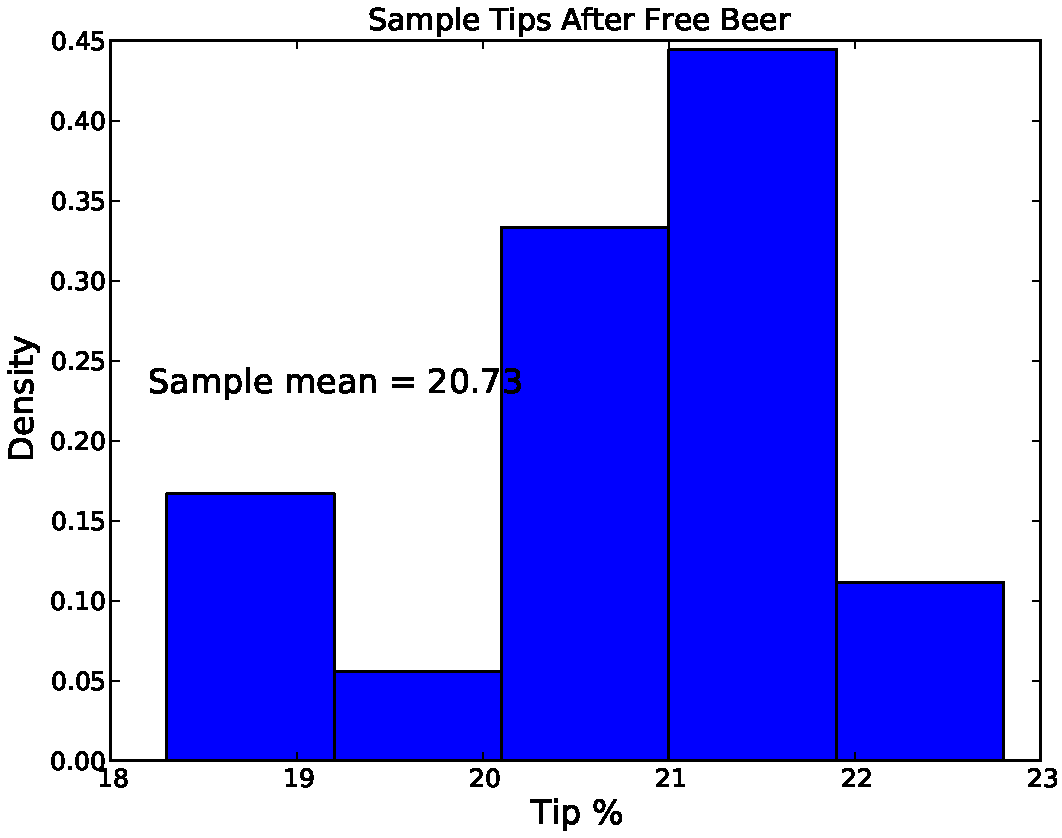
\includegraphics{figures/tips-histo.pdf}}

For your convenience, here are the tips in python format:

\begin{pyverbatim}
tips = [20.8, 18.7, 19.1, 20.6, 21.9, 20.4, 22.8,
        21.9, 21.2, 20.3, 21.9, 18.3, 21.0, 20.3,
        19.2, 20.2, 21.1, 22.1, 21.0, 21.7]
\end{pyverbatim}

(Use your awesome new skills from previous labs to generate the histogram.) To me, there is a lot of ``mass'' to the right of the usual 20\% tip but my eyeball is not a rigorous significance mechanism. 

\step To get a better idea, let's simply plot the distribution of the sample means given our $H_0$ assumption: $N(0.20, s^2/n)$. This is our ``control'' or the usual tipping distribution: the distribution of the set of average tips per day if $H_0$, the control, is true.

\scalebox{.45}{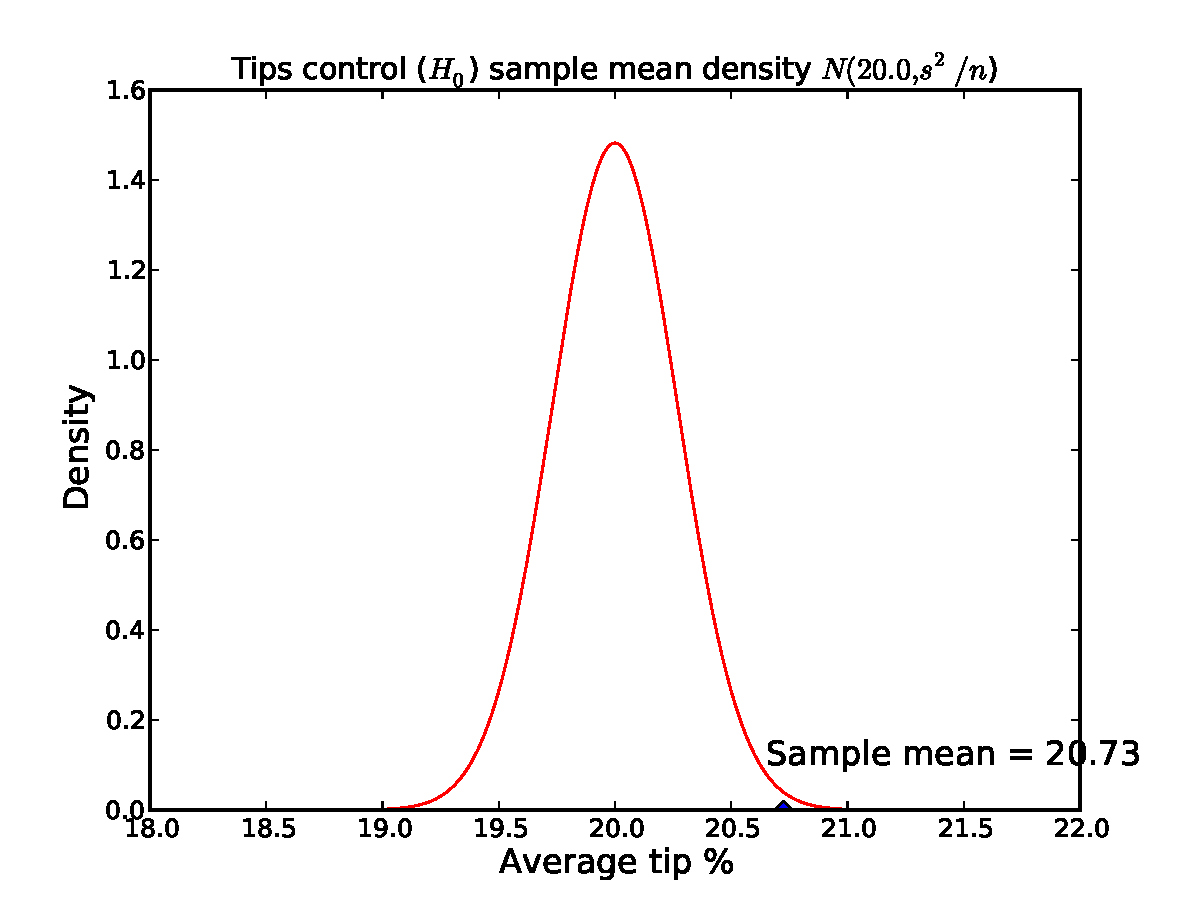
\includegraphics{figures/tips-means-dist.pdf}}

Looking at that graph, it seems that a sample mean of 20.73 is pretty far in the right tail of a normal curve centered at the control average 20\% tip. It looks to be a few standard deviations away from the mean. My gut says that it's pretty likely that giving people a free beer increases tips significantly.

\subsection{t-test}

\setcounter{problem}{1}

\step Let's use a {\em t-test} now to test for significance, just like we would do in statistics class. The $t$ value measures the number of standard deviations a sample mean, $m$, is away from our presumed population mean $\mu$: \\

\[\tag{t-value}
t = \frac{m - \mu}{s / \sqrt{N}}
\]

\noindent It's just the difference between the means scaled to be in units of standard deviations.  Write some code to compute the t-value. When computing $s$, the sample standard deviation, note that the numpy std() function returns a biased estimate of the standard deviation. Use {\tt np.std(tips, ddof=1)} instead of just {\tt std(tips)}. Print out the value of $t$.

I get $t = 2.69417199392$. That means that $m$ is about 2.7 standard deviations away from $\mu$, which is a very significant departure. 

\step  To get a p-value, likelihood that we would see such a $t$ value in the nonfree beer situation, look up $t$ in a t-distribution c.d.f. using {\tt 1-stats.t.cdf(t,N-1)}. You should get $0.0071844$. Since we need to check both tails, the probability is actually $2x$ that, or, p-value=$0.014369$ (1.4\%). The definition of significance is $\alpha = 0.06$, which means that our sample mean is definitely significant since $1.4\% < 6\%$.  There is only a 1.4\% chance that the control could generate a value that extreme or beyond.

We must conclude that $m$ differs significantly from $\mu = 0.20$ based upon the significance of $\alpha=0.06$ and, therefore, we reject $H_0$ in favor of $H_1$.  Giving out free beers is extremely likely to have increased the average tip in that experiment.

\subsection{Boostrapping for empirical hypothesis testing}

\setcounter{problem}{1}

Ok, now, let's use bootstrapping to estimate a {\em p-value}. A p-value for some point statistic or value is the probability that the control (null hypothesis $H_0$) could generate that statistic or value. In our case, a p-value can tell us the likelihood that a normal distribution centered around $\mu=20.0$ with $s^2=var(tips)$ could generate a sample mean of 20.725. (We approximate the population variance with our sample variance.) Note and we are sampling from $N(\mu,s^2)$ not resampling from the tips list as we are trying to see how the observed sample mean fits within the controlled distribution.

\step Bootstrap TRIALS samples of size $n=len(tips)$ from $N(\mu, s^2)$. It's very important that we use the same sample size as $len(tips)$ so we are comparing the same thing. Recall that the variance of $\overline{X}$ is a function of $s^2/n$. Compute the mean of each sample, $X$, an add to $\overline{X}$ as you generate samples from the normal distribution.

\step Compute how many sample means are greater than or equal to mean(tips):

\begin{pyverbatim}
greater = np.sum(X_ > np.mean(tips))
\end{pyverbatim}

or

\begin{pyverbatim}
greater = sum([x>np.mean(tips) for x in X_]) # the number of true values
\end{pyverbatim}

\step The (one-sided) p-value is just the ratio of values above the observed mean, mean(tips), to the number of trials. Double that because we're doing a two-sided test. With 5000 trials, I see just 13 values greater than $m=20.725$. That gives us a p-value of 2*13/5000 = 0.0052 or .52\%. That means that, empirically, we find that there is an extremely small probability that the control could generate an extreme value like $m=20.725$. Certainly the likelihood is less than the required 6\% significant value. 

Note: we would expect the empirical p-value (.52\%) and the p-value derived from the t-test (1.4\%) to be very close to each other when the number of trials is large with bootstrapping.  Our resident statistician, Jeff Hamrick, explains that the difference is not a problem with our bootstrapping solution and is ok.

``{\em A student t distribution with dof=19, is pretty close to a normal. But the differences are most greatly felt in the tails, and we're in the tails (rejection $H_{0}$), thus casting a little bit of sketchiness or your choice to draw the simulated raw data from a normal random variable. If we were performing this exact same operation on a data set with reasonably large size (say, 40 or 50 or 75) the differences would still exist but be even more minute.}''

Again, we easily reject the control and conclude that giving out free beers increases tips.

\section{Deliverables}

Please submit:

\begin{itemize}
\item {\tt hyp.py}
\item a text file with your t-value, and p-value from the t-test. Also give your empirical p-value from bootstrapping with TRIALS=5000.
\end{itemize}

\end{fullwidth}
